\documentclass[12pt,a4paper]{article}

% ==================== PACKAGES ====================
\usepackage[utf8]{inputenc}
\usepackage[T1]{fontenc}
\usepackage{amsmath,amssymb,amsthm,amsfonts}
\usepackage{mathtools}
\usepackage{physics}
\usepackage{tikz}
\usepackage{tikz-3dplot}
\usetikzlibrary{arrows,decorations.markings,calc,positioning,shapes.geometric}
\usepackage{graphicx}
\usepackage{hyperref}
\usepackage{geometry}
\usepackage{fancyhdr}
\usepackage{xcolor}
\usepackage{tcolorbox}
\usepackage{float}
\usepackage{caption}
\usepackage{subcaption}
\usepackage{enumitem}

\geometry{margin=1in}

% ==================== THEOREM ENVIRONMENTS ====================
\theoremstyle{definition}
\newtheorem{definition}{Definition}[section]
\newtheorem{theorem}{Theorem}[section]
\newtheorem{lemma}[theorem]{Lemma}
\newtheorem{proposition}[theorem]{Proposition}
\newtheorem{corollary}[theorem]{Corollary}
\newtheorem{example}{Example}[section]
\newtheorem{remark}{Remark}[section]

% ==================== CUSTOM COMMANDS ====================
\newcommand{\C}{\mathbb{C}}
\newcommand{\R}{\mathbb{R}}
\newcommand{\CP}{\mathbb{CP}}
\newcommand{\Z}{\mathbb{Z}}
\newcommand{\N}{\mathbb{N}}
\newcommand{\SU}{\mathrm{SU}}
\newcommand{\SO}{\mathrm{SO}}
\newcommand{\SL}{\mathrm{SL}}
\newcommand{\Spin}{\mathrm{Spin}}
\newcommand{\spinnet}{\mathcal{S}}
\newcommand{\twistor}{\mathcal{T}}
\newcommand{\hilbert}{\mathcal{H}}

% ==================== COLOR DEFINITIONS ====================
\definecolor{tealblue}{RGB}{0,128,128}
\definecolor{deepblue}{RGB}{0,51,102}
\definecolor{lightblue}{RGB}{173,216,230}

% ==================== TITLE CONFIGURATION ====================
\title{\textbf{\Huge Twistor Theory and Spin Networks}\\
\vspace{0.5cm}
\Large A Comprehensive Mathematical Visualization}
\author{Generated Visualization Framework}
\date{\today}

% ==================== DOCUMENT BEGIN ====================
\begin{document}

\maketitle
\tableofcontents
\newpage

% ==================== ABSTRACT ====================
\begin{abstract}
This document provides a comprehensive mathematical treatment of twistor theory and spin networks, two fundamental frameworks in modern theoretical physics. Twistor theory, introduced by Roger Penrose, reformulates spacetime geometry in terms of complex projective geometry. Spin networks, developed in the context of loop quantum gravity, provide a discrete description of quantum geometry. We present detailed mathematical foundations, visualizations, and connections between these two frameworks.
\end{abstract}

% ==================== SECTION 1: INTRODUCTION ====================
\section{Introduction}

\subsection{Motivation}
The quest to unify general relativity with quantum mechanics has led to revolutionary mathematical frameworks. Two of the most elegant approaches are:

\begin{itemize}[leftmargin=*]
    \item \textbf{Twistor Theory}: A geometric approach that encodes spacetime structure in terms of complex geometry
    \item \textbf{Spin Networks}: A combinatorial-algebraic framework describing quantum states of geometry
\end{itemize}

\subsection{Historical Context}
\begin{tcolorbox}[colback=lightblue!10,colframe=deepblue,title=Historical Timeline]
\begin{itemize}
    \item \textbf{1967}: Roger Penrose introduces twistor theory
    \item \textbf{1971}: Penrose and MacCallum develop twistor diagram formalism
    \item \textbf{1988}: Rovelli and Smolin introduce spin networks
    \item \textbf{1995}: Connection between twistors and spin networks discovered
    \item \textbf{2004}: Witten connects twistor strings to gauge theory
\end{itemize}
\end{tcolorbox}

% ==================== SECTION 2: TWISTOR THEORY ====================
\section{Twistor Theory}

\subsection{Mathematical Foundations}

\begin{definition}[Twistor Space]
The \emph{projective twistor space} $\mathbb{PT}$ is the complex projective 3-space $\CP^3$. A twistor $Z^\alpha$ is a homogeneous coordinate on $\mathbb{PT}$, represented as:
\begin{equation}
Z^\alpha = \begin{pmatrix} \omega^A \\ \pi_{A'} \end{pmatrix}, \quad \alpha = 0,1,2,3
\end{equation}
where $\omega^A$ ($A=0,1$) are spinor components and $\pi_{A'}$ ($A'=0',1'$) are conjugate spinor components.
\end{definition}

\begin{definition}[Incidence Relations]
A point $x^{AA'}$ in complexified Minkowski space $\C M$ corresponds to a line (projective line) in twistor space via the incidence relation:
\begin{equation}
\omega^A = ix^{AA'}\pi_{A'}
\end{equation}
This establishes the twistor correspondence between spacetime points and $\CP^1$ subspaces of $\CP^3$.
\end{definition}

\subsection{Spinor Formalism}

The foundation of twistor theory lies in the spinor representation of the Lorentz group.

\begin{theorem}[Spinor Decomposition]
The Lorentz group $\SO(3,1)$ has a double cover $\SL(2,\C)$. Any spacetime vector $x^\mu$ can be decomposed as:
\begin{equation}
x^{AA'} = \frac{1}{\sqrt{2}}\sigma^\mu_{AA'} x_\mu
\end{equation}
where $\sigma^\mu_{AA'}$ are the Infeld-van der Waerden symbols.
\end{equation}
\end{theorem}

\subsection{Penrose Transform}

\begin{tcolorbox}[colback=tealblue!5,colframe=tealblue,title=The Penrose Transform]
The Penrose transform is a correspondence between:
\begin{align}
H^1(\mathbb{PT}, \mathcal{O}(-n-2)) &\longleftrightarrow \text{Zero-rest-mass fields of helicity } n/2\\
\text{Cohomology on twistor space} &\longleftrightarrow \text{Physical fields on spacetime}
\end{align}
\end{tcolorbox}

\subsection{Twistor Geometry Visualization}

\begin{figure}[H]
\centering
\begin{tikzpicture}[scale=1.5]
    % Twistor space representation
    \draw[thick,->] (0,0) -- (3,0) node[right] {$\omega^0$};
    \draw[thick,->] (0,0) -- (0,3) node[above] {$\omega^1$};
    \draw[thick,->] (0,0) -- (-1.5,-1.5) node[left] {$\pi_0$};
    
    % Complex projective space
    \draw[blue,thick] (1.5,1.5) circle (1.2cm);
    \node[blue] at (1.5,3) {$\CP^3$};
    
    % Correspondence lines
    \foreach \x in {0.5,1,1.5,2,2.5} {
        \draw[red,dashed,opacity=0.6] (\x,0) -- (\x,2.5);
    }
    
    % Labels
    \node at (4.5,2) {Twistor Space};
    \draw[thick,->] (4.5,1.5) -- (4.5,0.5);
    \node at (4.5,0) {Spacetime};
    
    % Spacetime point
    \fill[green] (1.5,1.5) circle (2pt);
    \node[green,right] at (1.5,1.5) {$x^{AA'}$};
\end{tikzpicture}
\caption{Schematic representation of twistor space $\CP^3$ and its correspondence to spacetime points}
\end{figure}

\subsection{Alpha-Plane and Beta-Plane}

\begin{definition}[Alpha-Planes and Beta-Planes]
\begin{itemize}
    \item An \textbf{$\alpha$-plane} in twistor space corresponds to a point in spacetime
    \item A \textbf{$\beta$-plane} in twistor space corresponds to a null ray in spacetime
\end{itemize}
\end{definition}

\begin{equation}
\begin{aligned}
\text{$\alpha$-plane:} &\quad \omega^A = ix^{AA'}\pi_{A'} \\
\text{$\beta$-plane:} &\quad \pi_{A'} = iy_{A'A}\omega^A
\end{aligned}
\end{equation}

% ==================== SECTION 3: SPIN NETWORKS ====================
\section{Spin Networks}

\subsection{Basic Structure}

\begin{definition}[Spin Network]
A \emph{spin network} is a directed graph $\Gamma = (V, E)$ where:
\begin{itemize}
    \item $V$ is the set of vertices (nodes)
    \item $E$ is the set of edges
    \item Each edge $e \in E$ is labeled by a spin $j_e \in \{0, 1/2, 1, 3/2, \ldots\}$
    \item Each vertex $v \in V$ is labeled by an intertwiner $\iota_v \in \mathrm{Inv}(\bigotimes_{e \sim v} V_{j_e})$
\end{itemize}
\end{definition}

\subsection{Mathematical Framework}

\begin{theorem}[Spin Network States]
A spin network state $|\Gamma, j_e, \iota_v\rangle$ defines a quantum state of geometry. The Hilbert space of quantum geometry is:
\begin{equation}
\hilbert_{\text{spin}} = \bigoplus_{\Gamma} \bigotimes_{e \in E(\Gamma)} \hilbert_{j_e}
\end{equation}
where $\hilbert_{j_e}$ is the $(2j_e+1)$-dimensional representation space of $\SU(2)$.
\end{theorem}

\subsection{Geometric Interpretation}

\begin{tcolorbox}[colback=lightblue!10,colframe=deepblue,title=Physical Interpretation]
\begin{itemize}
    \item \textbf{Edges}: Represent quantized areas (flux of area operators)
    \item \textbf{Vertices}: Represent quantized volumes
    \item \textbf{Spin labels $j$}: Encode area eigenvalues $A = 8\pi\gamma\ell_P^2\sqrt{j(j+1)}$
\end{itemize}
where $\gamma$ is the Immirzi parameter and $\ell_P$ is the Planck length.
\end{tcolorbox}

\subsection{Visualization of Simple Spin Networks}

\begin{figure}[H]
\centering
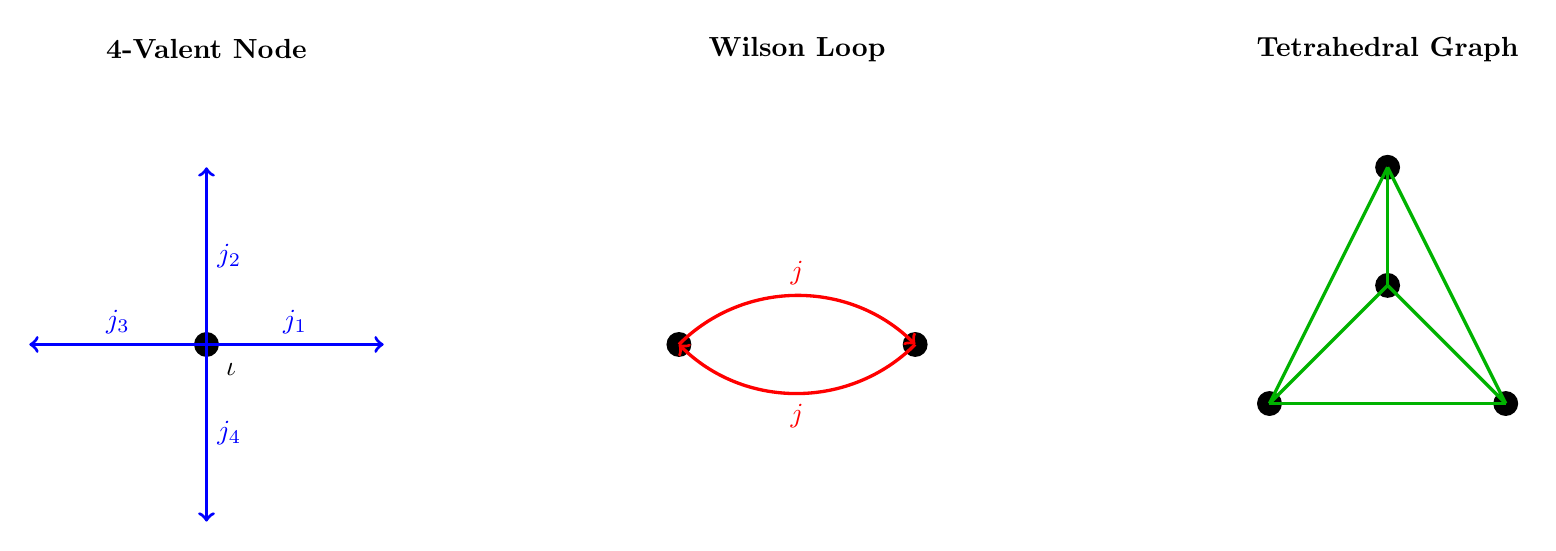
\begin{tikzpicture}[scale=1.5]
    % 4-valent vertex
    \begin{scope}
        \node at (0,2.5) {\textbf{4-Valent Node}};
        \coordinate (center) at (0,0);
        \fill (center) circle (3pt);
        
        % Four edges
        \draw[very thick,blue,->] (center) -- (1.5,0) node[midway,above] {$j_1$};
        \draw[very thick,blue,->] (center) -- (0,1.5) node[midway,right] {$j_2$};
        \draw[very thick,blue,->] (center) -- (-1.5,0) node[midway,above] {$j_3$};
        \draw[very thick,blue,->] (center) -- (0,-1.5) node[midway,right] {$j_4$};
        
        \node at (center) [below right=5pt] {$\iota$};
    \end{scope}
    
    % Simple loop
    \begin{scope}[xshift=5cm]
        \node at (0,2.5) {\textbf{Wilson Loop}};
        \coordinate (v1) at (-1,0);
        \coordinate (v2) at (1,0);
        
        \fill (v1) circle (3pt);
        \fill (v2) circle (3pt);
        
        \draw[very thick,red,->] (v1) to[bend left=45] node[midway,above] {$j$} (v2);
        \draw[very thick,red,->] (v2) to[bend left=45] node[midway,below] {$j$} (v1);
    \end{scope}
    
    % Tetrahedron graph
    \begin{scope}[xshift=10cm]
        \node at (0,2.5) {\textbf{Tetrahedral Graph}};
        \coordinate (A) at (0,1.5);
        \coordinate (B) at (-1,-0.5);
        \coordinate (C) at (1,-0.5);
        \coordinate (D) at (0,0.5);
        
        \fill (A) circle (3pt);
        \fill (B) circle (3pt);
        \fill (C) circle (3pt);
        \fill (D) circle (3pt);
        
        \draw[very thick,green!70!black] (A) -- (B);
        \draw[very thick,green!70!black] (B) -- (C);
        \draw[very thick,green!70!black] (C) -- (A);
        \draw[very thick,green!70!black] (D) -- (A);
        \draw[very thick,green!70!black] (D) -- (B);
        \draw[very thick,green!70!black] (D) -- (C);
    \end{scope}
\end{tikzpicture}
\caption{Examples of spin network structures: (left) 4-valent vertex with intertwiner, (center) Wilson loop configuration, (right) tetrahedral graph structure}
\end{figure}

\subsection{Recoupling Theory and 6j-Symbols}

\begin{definition}[Wigner 6j-Symbol]
The Wigner 6j-symbol encodes the recoupling coefficients for angular momentum:
\begin{equation}
\begin{Bmatrix}
j_1 & j_2 & j_{12} \\
j_3 & j & j_{23}
\end{Bmatrix}
= \sum_m (-1)^{j+m} \langle j_1 j_2 j_{12} | j_3 m \rangle \langle j_{23} j_3 m | j_1 j_2 \rangle
\end{equation}
These appear in spin network evaluations at vertices.
\end{definition}

\begin{figure}[H]
\centering
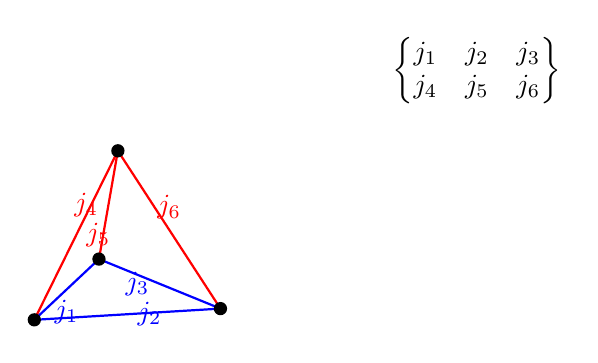
\begin{tikzpicture}[scale=1.2]
    % 6j-symbol as tetrahedron
    \tdplotsetmaincoords{70}{110}
    \begin{scope}[tdplot_main_coords]
        \coordinate (A) at (0,0,0);
        \coordinate (B) at (2,0,0);
        \coordinate (C) at (1,1.732,0);
        \coordinate (D) at (1,0.577,1.633);
        
        % Draw edges
        \draw[thick,blue] (A) -- (B) node[midway,below] {$j_1$};
        \draw[thick,blue] (B) -- (C) node[midway,right] {$j_2$};
        \draw[thick,blue] (C) -- (A) node[midway,left] {$j_3$};
        \draw[thick,red] (A) -- (D) node[midway,left] {$j_4$};
        \draw[thick,red] (B) -- (D) node[midway,right] {$j_5$};
        \draw[thick,red] (C) -- (D) node[midway,above] {$j_6$};
        
        % Draw vertices
        \foreach \point in {A,B,C,D} {
            \fill (\point) circle (2pt);
        }
    \end{scope}
    
    \node at (4,2) {$\begin{Bmatrix} j_1 & j_2 & j_3 \\ j_4 & j_5 & j_6 \end{Bmatrix}$};
\end{tikzpicture}
\caption{Geometric representation of 6j-symbol as tetrahedral graph}
\end{figure}

% ==================== SECTION 4: CONNECTIONS ====================
\section{Connections Between Twistors and Spin Networks}

\subsection{Unifying Framework}

Both twistor theory and spin networks provide reformulations of spacetime geometry:

\begin{table}[H]
\centering
\begin{tabular}{|l|l|l|}
\hline
\textbf{Aspect} & \textbf{Twistor Theory} & \textbf{Spin Networks} \\
\hline
Fundamental object & Complex lines in $\CP^3$ & Graphs with $\SU(2)$ labels \\
\hline
Spacetime picture & Emergent from twistor geometry & Discrete quantum geometry \\
\hline
Symmetry group & $\SL(2,\C)$ & $\SU(2)$ \\
\hline
Physical regime & Classical + massless fields & Quantum gravity \\
\hline
Dimensional & 4D continuous & 3D discrete \\
\hline
\end{tabular}
\caption{Comparison of twistor theory and spin networks}
\end{table}

\subsection{Spinor Networks as Bridge}

\begin{proposition}[Spinor Network Correspondence]
There exists a correspondence between:
\begin{itemize}
    \item Spin network states with $\SU(2)$ labels
    \item Twistor diagrams with spinor indices
    \item Both encode the same kinematical structure of quantum geometry
\end{itemize}
\end{proposition}

\subsection{Holomorphic Linking}

\begin{definition}[Holomorphic Curves in Twistor Space]
A holomorphic curve $\mathcal{C} \subset \mathbb{PT}$ corresponds to an extended object in spacetime. Linking numbers of such curves relate to spin network evaluations:
\begin{equation}
\langle \Gamma_1 | \Gamma_2 \rangle = \oint_{\mathcal{C}_1} \oint_{\mathcal{C}_2} K(Z_1, Z_2)
\end{equation}
where $K$ is the twistor linking kernel.
\end{definition}

% ==================== SECTION 5: ADVANCED TOPICS ====================
\section{Advanced Topics}

\subsection{Quantum Corrections and Foam}

\begin{tcolorbox}[colback=tealblue!5,colframe=tealblue,title=Spin Foam Models]
Spin foams extend spin networks by describing spacetime evolution:
\begin{itemize}
    \item \textbf{Faces}: Labeled by spins $j_f$ (2D surfaces)
    \item \textbf{Edges}: Labeled by intertwiners (1D curves)
    \item \textbf{Vertices}: Labeled by amplitudes (0D points)
\end{itemize}

The amplitude for a spin foam $\mathcal{F}$ is:
\begin{equation}
Z(\mathcal{F}) = \sum_{\{j_f\}} \prod_{f} (2j_f+1) \prod_{e} A_e(j_f) \prod_{v} A_v(j_f, \iota_e)
\end{equation}
\end{tcolorbox}

\subsection{Twistor Strings}

\begin{remark}[Witten's Twistor String Theory]
Edward Witten showed that $\mathcal{N}=4$ super Yang-Mills theory can be described by a string theory in twistor space, connecting:
\begin{equation}
\text{Gauge theory amplitudes} \longleftrightarrow \text{String amplitudes on } \CP^{3|4}
\end{equation}
\end{remark}

\subsection{Black Hole Entropy from Spin Networks}

\begin{theorem}[Bekenstein-Hawking from Spin Networks]
The entropy of a black hole horizon of area $A$ can be computed by counting spin network states piercing the horizon:
\begin{equation}
S_{BH} = \frac{k_B A}{4\ell_P^2} = k_B \sum_p \ln\left(2j_p + 1\right)
\end{equation}
where the sum is over punctures with spin $j_p$.
\end{theorem}

% ==================== SECTION 6: COMPUTATIONAL EXAMPLES ====================
\section{Computational Examples}

\subsection{Computing Spin Network Evaluations}

\begin{example}[Theta Graph Evaluation]
Consider a theta graph with three edges connecting two vertices:

\begin{center}
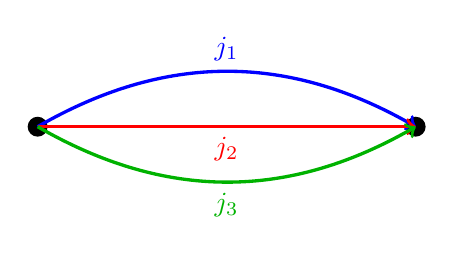
\begin{tikzpicture}[scale=1.2]
    \coordinate (L) at (0,0);
    \coordinate (R) at (4,0);
    
    \fill (L) circle (3pt);
    \fill (R) circle (3pt);
    
    \draw[very thick,blue,->] (L) to[bend left=30] node[midway,above] {$j_1$} (R);
    \draw[very thick,red,->] (L) -- node[midway,below] {$j_2$} (R);
    \draw[very thick,green!70!black,->] (L) to[bend right=30] node[midway,below] {$j_3$} (R);
\end{tikzpicture}
\end{center}

The evaluation involves computing:
\begin{equation}
\langle \Gamma_\theta \rangle = \sum_{m_1,m_2,m_3} C^{j_1 j_2 j_3}_{m_1 m_2 m_3} C^{j_1 j_2 j_3}_{m_1 m_2 m_3}
\end{equation}
where $C$ are Clebsch-Gordan coefficients.
\end{example}

\subsection{Area Spectrum}

\begin{example}[Quantized Area]
For a surface $S$ pierced by $n$ spin network edges with spins $\{j_1, j_2, \ldots, j_n\}$:
\begin{equation}
A_S = 8\pi\gamma\ell_P^2 \sum_{i=1}^n \sqrt{j_i(j_i+1)}
\end{equation}

For $n=3$ with spins $(1/2, 1, 1/2)$:
\begin{align}
A_S &= 8\pi\gamma\ell_P^2 \left[\sqrt{\frac{1}{2} \cdot \frac{3}{2}} + \sqrt{1 \cdot 2} + \sqrt{\frac{1}{2} \cdot \frac{3}{2}}\right] \\
&= 8\pi\gamma\ell_P^2 \left[\frac{\sqrt{3}}{2} + \sqrt{2} + \frac{\sqrt{3}}{2}\right] \\
&= 8\pi\gamma\ell_P^2 (\sqrt{3} + \sqrt{2})
\end{align}
\end{example}

% ==================== SECTION 7: FUTURE DIRECTIONS ====================
\section{Future Directions}

\subsection{Open Problems}

\begin{enumerate}
    \item \textbf{Semiclassical limit}: How do spin networks reproduce smooth spacetime?
    \item \textbf{Twistor quantization}: Can twistor theory be fully quantized?
    \item \textbf{Matter coupling}: How to incorporate matter fields?
    \item \textbf{Cosmological constant}: Role of $\Lambda$ in both frameworks
    \item \textbf{Unification}: Complete dictionary between twistors and spin networks
\end{enumerate}

\subsection{Recent Developments}

\begin{itemize}
    \item Amplituhedron and positive geometry
    \item Holographic spin networks
    \item Twistor formulations of QFT
    \item Quantum information perspectives
\end{itemize}

% ==================== REFERENCES ====================
\section{References}

\begin{enumerate}
    \item Penrose, R. (1967). \emph{Twistor algebra}. Journal of Mathematical Physics, 8(2), 345-366.
    \item Penrose, R., \& Rindler, W. (1984). \emph{Spinors and space-time} (Vol. 1). Cambridge University Press.
    \item Rovelli, C., \& Smolin, L. (1995). \emph{Spin networks and quantum gravity}. Physical Review D, 52(10), 5743.
    \item Baez, J. C. (1996). \emph{Spin network states in gauge theory}. Advances in Mathematics, 117(2), 253-272.
    \item Witten, E. (2004). \emph{Perturbative gauge theory as a string theory in twistor space}. Communications in Mathematical Physics, 252(1-3), 189-258.
    \item Rovelli, C. (2004). \emph{Quantum Gravity}. Cambridge University Press.
    \item Penrose, R. (2005). \emph{The Road to Reality}. Jonathan Cape.
    \item Ashtekar, A., \& Lewandowski, J. (2004). \emph{Background independent quantum gravity: A status report}. Classical and Quantum Gravity, 21(15), R53.
\end{enumerate}

% ==================== APPENDICES ====================
\appendix

\section{Spinor Conventions}

\subsection{Spinor Index Notation}
\begin{itemize}
    \item Unprimed indices: $A, B, C, \ldots = 0, 1$ (left-handed spinors)
    \item Primed indices: $A', B', C', \ldots = 0', 1'$ (right-handed spinors)
    \item Spinor metric: $\epsilon_{AB} = \begin{pmatrix} 0 & 1 \\ -1 & 0 \end{pmatrix}$
\end{itemize}

\subsection{Key Identities}
\begin{align}
\epsilon_{AB}\epsilon^{CD} &= \delta_A^C \delta_B^D - \delta_A^D \delta_B^C \\
\sigma^\mu_{AA'} \bar{\sigma}_\mu^{BB'} &= 2\delta_A^B \delta_{A'}^{B'}
\end{align}

\section{Representation Theory of SU(2)}

\subsection{Irreducible Representations}
For spin-$j$ representation ($j = 0, 1/2, 1, 3/2, \ldots$):
\begin{equation}
\dim V_j = 2j + 1
\end{equation}

\subsection{Clebsch-Gordan Decomposition}
\begin{equation}
V_{j_1} \otimes V_{j_2} = \bigoplus_{j=|j_1-j_2|}^{j_1+j_2} V_j
\end{equation}

\section{TikZ Code for Figures}

All figures in this document are generated using TikZ. The source code is embedded directly in the LaTeX source and can be extracted and modified for custom visualizations.

% ==================== END DOCUMENT ====================
\end{document}
